\begin{figure}[!t]
\centering
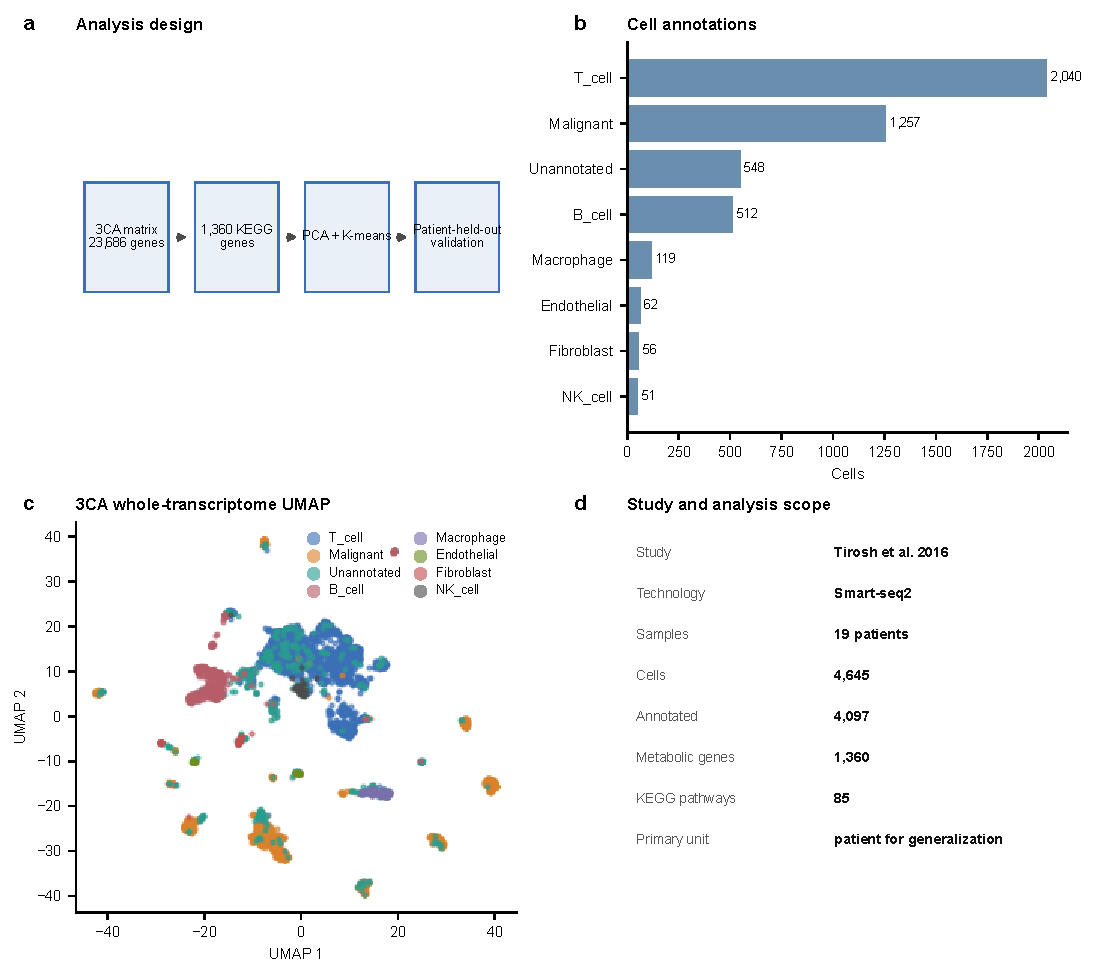
\includegraphics[width=\textwidth]{../results/figures/figure1_dataset_and_design.pdf}
\caption{Dataset and analysis design. (a) Analysis design overview: 4,645 cells from 19 melanoma samples analyzed using 1,360 metabolic genes from KEGG pathways. (b) Cell annotation counts: 4,097 annotated cells, 548 unannotated cells. (c) UMAP embedding of cells colored by annotation, using 3CA-provided whole-transcriptome coordinates; metabolic gene re-fitting was not performed on this embedding. (d) Study scope: 19 patients, 4,645 cells total, 1,360 metabolic genes.}
\label{fig:dataset}
\end{figure}

\begin{figure}[!t]
\centering
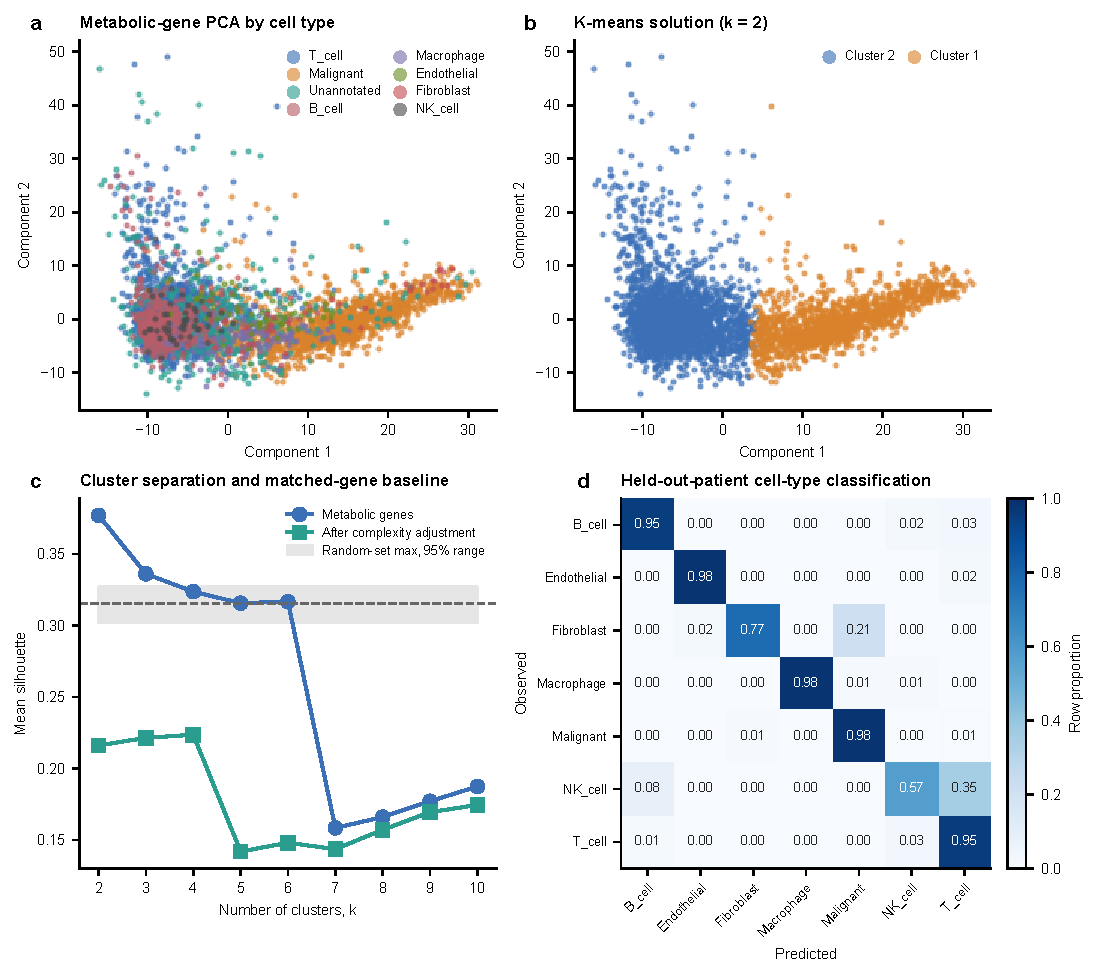
\includegraphics[width=\textwidth]{../results/figures/figure2_metabolic_separation.pdf}
\caption{Metabolic gene separation. (a) PCA of 1,360 metabolic genes on 4,645 cells, colored by cell type. (b) Same PCA colored by k-means cluster assignment at k = 2. (c) Silhouette scores across k = 2..10 for all cells, with raw and complexity-adjusted curves; the 95\% empirical range of 20 matched random gene sets is shown as a shaded band (not a confidence interval, not an HVG result). (d) Patient-blocked 5-fold cross-validation on 4,097 annotated cells using pooled row-normalized data, showing confusion matrix for cell-type classification.}
\label{fig:separation}
\end{figure}

\begin{figure}[!t]
\centering
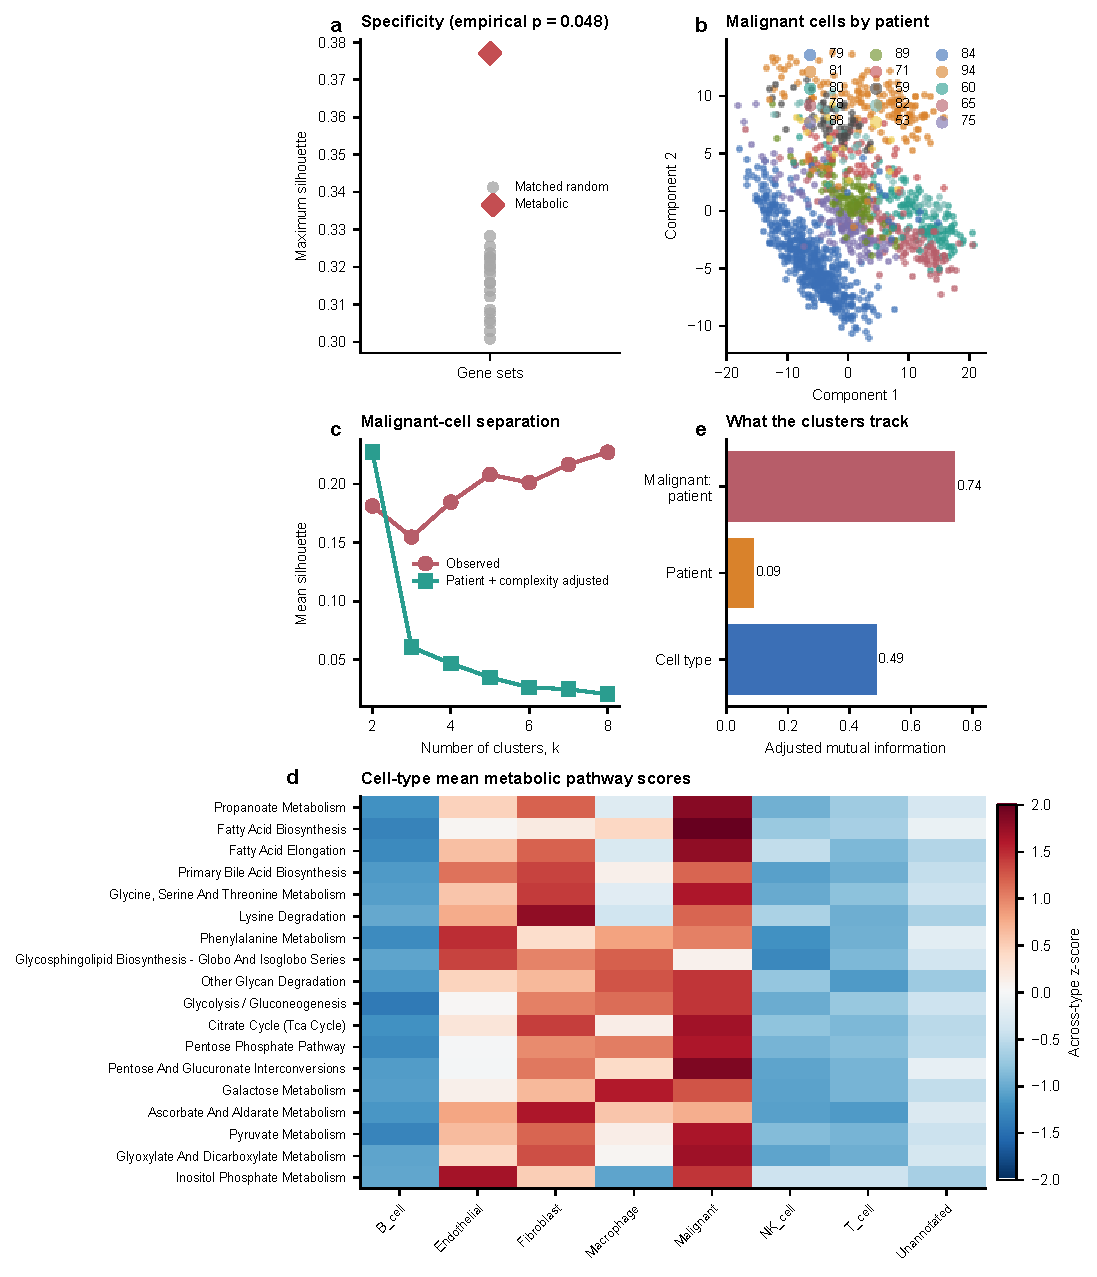
\includegraphics[width=\textwidth]{../results/figures/figure3_robustness_and_interpretation.pdf}
\caption{Robustness and interpretation. (a) All-cell maximum silhouette comparison of 20 matched random gene sets against the metabolic gene set. (b) PCA of 1,257 malignant cells colored by patient, showing patient-level clustering. (c) Silhouette curves for malignant cells across k = 2..8, with raw and patient+complexity-adjusted curves. (d) Heatmap of 18 KEGG metabolic pathway z-scores across cell types, showing across-type mean scores (not flux or scMetabolism scoring). (e) Adjusted mutual information (AMI) for alignment with cell type, patient, and malignant patient, comparing all-cell, all-patient, and malignant-patient analyses.}
\label{fig:robustness}
\end{figure}
